\documentclass{proc}
\usepackage{graphicx}
\usepackage{mathtools}
\usepackage{fixltx2e}
\usepackage{algorithm}
\usepackage{algpseudocode}
\usepackage{caption}
\usepackage{url}
\usepackage{amsmath}
\usepackage{mathrsfs}
\usepackage{tikz}
\usetikzlibrary{positioning}
\setlength{\abovecaptionskip}{2pt}
\setcounter{secnumdepth}{2}

\title{
The Small World Network Effect in Software Project Teams
\author{Kevin Peterson\\
\small \texttt{pete1968@umn.edu}
}
}

\begin{document}
\maketitle

\begin{abstract}
Team cohesion and the dynamics of team forming are important parts of any project, with software projects being no exception. An interesting aspect of team building is the relationships formed between the team members. Because of these relationships, visualizing software team members as a graph may be a natural way to explore these relationships. As team members move between projects, these graphs become more and more connected as team members collaborate and form relationships. We show that this connectivity, known as the ``small world effect," has a positive impact on team performance when the connectivity levels are moderate. Performance degrades, however, at both very high and very low levels of connectivity. This aligns with similar research findings of non-software teams.
\end{abstract}

\noindent \\\textbf{Keywords.} Small World, Project Management, Software

\section{Introduction}
A social network is a graph of people and the connections between them. The dynamics of social networks have proved to be an important research topic for many different areas of study, from academic publication\cite{barabasi2002evolution}, to the success of Broadway musicals\cite{uzzi2005collaboration}. In general, a social network is important to understanding how ideas and influence are spread\cite{kempe2003maximizing}. Given that, we can begin to investigate the best conditions for optimal group performance within these networks.

A ``small world'' network is a social network characterized by high clustering of graph nodes paired with a short average path between nodes\cite{watts1998collective}. ``Clustering'' in this context means how closely nodes in the graph are related to each other, or ``the friend of my friend is also my friend.'' ``Average path length'' is the the shortest route between all possible nodes, averaged over the entire graph. Milgram, in his seminal study, found that any two people are linked through a chain of friends and acquaintances on average of 6 people long\cite{milgram1967small}, or in other words, the average path length between any two people.

Uzzi \cite{uzzi2005collaboration} expanded on this by exploring how these small world networks correlate to collaboration and creativity. In his study, the network of artists involved in the making of Broadway musicals from 1945 to 1989 were studied. Performance was then measured based on financial success and critical acclaim, and statistically compared to the clustering and path length of the graph.

We follow Uzzi's work, and expand it to software teams. We hypothesize that the qualities of a small world graph that foster collaboration, creativity, and the efficiency of how knowledge is transfered\cite{latora2001efficient} will also apply to software project teams. In this work, we investigate the ``small world'' phenomenon quantitatively by exploring open source project data, and qualitatively by a series of interviews of subject matter experts, and look to compare Uzzi's findings to ours.

\subsection{Hypothesis}
The formalization of the ``small world'' quality of a graph can be expressed by the \textit{Small World Quotient}, or $Q$\cite{watts1999small,watts1998collective}. The value $Q$ is calculated by dividing the clustering factor of graph by the average path length between nodes. Uzzi explored this value in graphs of Broadway productions\cite{uzzi2005collaboration}. His findings suggest that the success of Broadway productions is greatest when teams have a good mix of new and familiar members. Productions are less likely to be successful when team members are very familiar with each other. Also, probability of success drops much the same way when there is little familiarity between team members. This indicates that there is an optimal ratio of new and familiar members on a team -- or, an optimal value of $Q$ when related to performance.

\textit{Software Project Teams will perform best at moderate levels of $Q$. This performance, measured by the amount of interest their projects generate, will increase as the level of $Q$ increases for the contributor graph. This will continue up to an optimal $Q$ value, after which performance will begin to degrade. Thus, the performance curve given $Q$ will be inverse U-shaped, and match Uzzi's findings\cite{uzzi2005collaboration}.}

\section{Methods}

\subsection{Collection and Storage}
Data was collected using the freely available FLOSSmole\cite{floss2006} data sets of free and open source projects. Two datasets were analyzed -- data from from the popular open source project site \textit{Freecode}\footnote{http://freecode.com/}, and another from open source software repository \textit{SourceForge}\footnote{http://sourceforge.net/}. The Freecode dataset contained data up to September, 2013, while the SourceForge dataset was slightly older with data gathered on June 2009. Both datasets were chosen because they met two basic criteria: (1) they contained an exhaustive list of projects and contributors to those projects, and (2) they provided some sort of quantitative measure of project ``popularity." This popularity metric will be further described in sections below. Results were analyzed using the Python graph processing packaged NetworkX\cite{hagberg-2008-exploring}. All source code pertaining to the collection and analysis can be found at \url{https://github.com/kevinpeterson/small-world-effect-research}.

\subsection{Analysis}
The collected data was organized into a graph structure, with the nodes representing the contributors and the edges representing one or more shared project between contributors. For our purposes, ``contributors'' includes any person that has been identified as being associated with the project by the project hosting site (Freecode and SourceForge, for our purposes). It is important to note that ``contributor'' does not always imply code contributions -- as issue reporting and documentation, among other things, are valid contributions. Various properties of the graph were analyzed, followed by a qualitative section to help link the quantitative analysis to subject matter expert experiences.

\subsubsection{Graph Structure}
For each dataset, we first considered the dataset to be one large graph. It was observed that the contributor graph was ``disconnected,'' meaning that there was not a path between all possible nodes. From this large disconnected graph, we can extract a set of connected subgraphs, where each connected subgraph was analyzed. Metrics were then computed for each of these subgraphs. In order to correctly compute the metrics below, a minimum subgraph size was required. Specifically, many of the graph metrics of interest measured ``triangles'' of nodes and their connections. This implies a subgraph of {$>= 3$} nodes is needed. Subgraphs of {$< 3$} nodes were not considered for analysis.

\begin{figure}
\centering
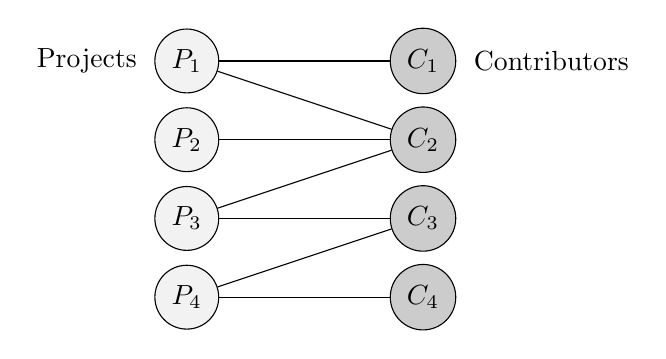
\begin{tikzpicture}
\tikzset{P/.style={circle,draw=black,fill=lightgray!20}}
\tikzset{C/.style={circle,draw=black,fill=black!20}}

 [scale=.5,auto=left]
  \node[P] (p1) at (-5,3)  {$P_1$};
  \node[P] (p2) at (-5,2)  {$P_2$};
  \node[P] (p3) at (-5,1)  {$P_3$};
  \node[P] (p4) at (-5,0)  {$P_4$};

  \node[C] (c1) at (-2,3)  {$C_1$};
  \node[C] (c2) at (-2,2)  {$C_2$};
  \node[C] (c3) at (-2,1)  {$C_3$};
  \node[C] (c4) at (-2,0)  {$C_4$};
  
  \draw ({p1}) -- ({c1});
  \draw ({p1}) -- ({c2});
  \draw ({p2}) -- ({c2});;
  \draw ({p3}) -- ({c2});
  \draw ({p3}) -- ({c3});
  \draw ({p4}) -- ({c3});
  \draw ({p4}) -- ({c4});
  \node[draw=none,fill=none,rectangle,left=1mm of p1] {Projects}; 
  \node[draw=none,fill=none,rectangle,right=1mm of c1] {Contributors}; 
\end{tikzpicture}
\caption{An example bipartite graph of Projects and Contributors}
\label{fig:example_bipartite_graph}
\end{figure}

The contributor/project data can be represented as a bipartite graph. A bipartite graph is a specialized type of graph containing two disjoint sets of verticies. This can be denoted by ${G=(P,C,E)}$, where ${P \cap C = \emptyset}$. For our purposes, let set $P$ be the set of all projects, and set $C$ be the set of all contributors. Each project node, therefore, is only connected to contributor nodes, and vice versa, as show in figure \ref{fig:example_bipartite_graph}. This bipartite representation is typical of what is found in social and collaboration networks\cite{ramasco2004self}.  

A bipartite graph projection is necessary to further analyze the graph. A bipartite projection involves taking the disjoint node sets $P$ and $C$, and representing the graph as relationships between only one of those sets of nodes. A projection onto the contributor nodes, or $C$, of figure \ref{fig:example_bipartite_graph} is show in figure \ref{fig:example_bipartite_projection_graph}. Here, contributors are connected directly, with edges occurring if a two contributors share one or more common projects. It is important to note that the projection could have been done in terms of the projects, not the contributors. This would have led to a graph with nodes of projects $P$, each being linked by sharing a common contributor. This approach is a common way of representing these bipartite graphs\cite{newman2001scientific}, although it is known that bipartite projections are lossy compared to the data represented in the original graph\cite{zhou2007bipartite}.\\

One of the main sources of information loss is multiple connections between contributors, or contributors that share multiple projects. When doing a bipartite projection based on contributors $C$, a single link could represent one shared project or many. This is a source of data loss in the projection. The simple approach is to treat one connection the same as many connections between nodes. This is straightforward but lossy\cite{zhou2007bipartite,grossman1995portion}. A better approach is to assign a \textit{weight} to each edge representing repeated links -- or in our case -- multiple shared collaborators\cite{zha2001bipartite,barrat2004architecture}.

\begin{figure}
\centering
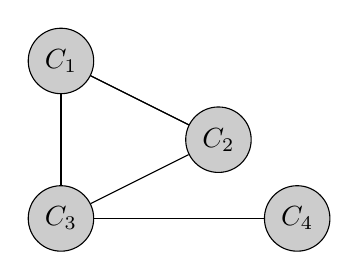
\begin{tikzpicture}
\tikzset{C/.style={circle,draw=black,fill=black!20}}

 [scale=.5,auto=left]
  \node[C] (c1) at (-5,3)  {$C_1$};
  \node[C] (c2) at (-3,2)  {$C_2$};
  \node[C] (c3) at (-5,1)  {$C_3$};
  \node[C] (c4) at (-2,1)  {$C_4$};

  \draw ({c1}) -- ({c3});
  \draw ({c1}) -- ({c2});
  \draw ({c1}) -- ({c2});
  \draw ({c2}) -- ({c3});
  \draw ({c3}) -- ({c4});
\end{tikzpicture}
\caption{A contributor ($C$) projection of the figure~\ref{fig:example_bipartite_graph} bipartite graph}
\label{fig:example_bipartite_projection_graph}
\end{figure}

\subsubsection{Graph Analysis}
To support our hypothesis, there are several key metrics to be studied in regards to the aforementioned graph. Many of these metrics follow the work of Boccaletti \textit{et. al}\cite{boccaletti2006complex}, and other studies of similar graph types\cite{latora2001efficient,adamic1999small}.

\noindent\\\textit{\textbf{Clustering Coefficient - Transitivity ($C^\Delta$)}}\\
We calculate the \textit{Clustering Coefficient} (or $C^\Delta$) as a measure of the proportion of closed triangles in a graph\cite{newman2003structure}:
\[C^\Delta = 3 \times \frac{\text{number of triangles}}
                    {\text{number of connected triples}}\]

This metric shows us how closely related, or ``clustered,'' that the graph is. It is also the probability that two nodes will be connected if they share a common neighbor\cite{newman2003properties}. In our context, if contributors $C_1$ and $C_2$ both collaborate with a common contributor w $C_3$, this metric represents the probability that $C_1$ and $C_2$ will collaborate.

\noindent\\\textit{\textbf{Clustering Coefficient - Average ($\overline{C^{\lambda}}$)}}\\
Another approach to clustering is to take the average of each node's local clustering coefficient\cite{watts1998collective}.

Given our graph of nodes $P$ connected by edges $E$, or ${G=(P,E)}$, for any given node we can determine its \textit{neighborhood} ($N_i$), or the set of nodes directly connected to a given node.
\[ N_i = \{v_j : e_{ij} \in E \wedge e_{ji} \in E \wedge v_j \in P\} \]

Given this \textit{neighborhood}, we can then calculate how closely connected the nodes are. To do this, we take the number of actual connections between neighbors divided by the total possible number of connections, where $k_i$ represents the count of the neighbors of a node, or {$k_i = |N_i|$}
\[ C^{\lambda}_i = \frac{2|\{e_{jk}: v_j,v_k \in N_i, e_{jk} \in E\}|}{k_i(k_i-1)} \]

From this \textit{Local Clustering Coefficient} $C_i$, we can then take the average over the entire set of nodes in the graph.
\[ \overline{C^\lambda} = \frac{1}{|P|}\sum^{|P|}_{i=1}C^{\lambda}_i \]

It is important to note that although the terminology is similar\cite{uzzi2005collaboration}, $\overline{C^\lambda}$ and $C^\Delta$ are different measurements. Unless otherwise noted, the Transitivity version of this metric ($C^\Delta$) will be used for all further calculations and metrics.

\noindent\\\textit{\textbf{Average Path Length ($L$)}}\\
Calculating the \textit{Path Length} ($L$) allowed us to determine how far removed contributors in the graph are from one another. The path length is calculated as the average distance between any two node pairs in the graph:

\[L = \frac{1}{|P| \cdot (|P|-1)} \sum_{i \neq j}\lambda(v_i,v_j)\]

Where {$v_i \in P$}, {$v_j \in P$}, and {$\lambda(v_i,v_j)$} denotes the shortest path between the two nodes. We only considered path length for connected subgraphs, avoiding some complexities of this calculation on disconnected graphs\cite{boccaletti2006complex}.

\begin{figure}
\centering
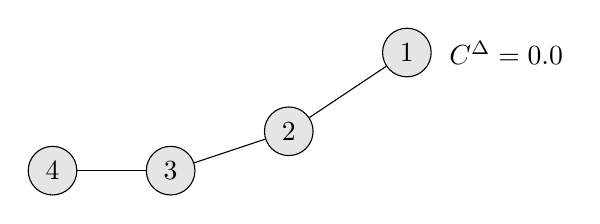
\begin{tikzpicture}
  [scale=.5,auto=left,every node/.style={circle,draw=black,fill=gray!20}]
  \node (n1) at (15,8) {1};
  \node (n2) at (12,6)  {2};
  \node (n3) at (9,5)  {3};
  \node (n4) at (6,5)  {4};
  \node[draw=none,fill=none,rectangle,right=1mm of n1] {$C^\Delta = 0.0$}; 
  
  \draw ({n1}) -- ({n2});
  \draw ({n2}) -- ({n3});
  \draw ({n3}) -- ({n4});
\end{tikzpicture}

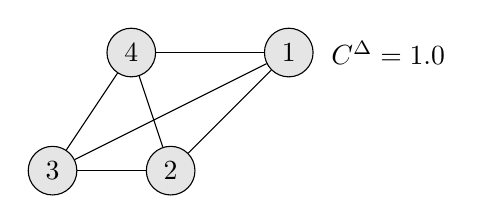
\begin{tikzpicture}
  [scale=.5,auto=left,every node/.style={circle,draw=black,fill=gray!20}]

  \node (n1) at (15,8) {1};
  \node (n2) at (12,5)  {2};
  \node (n3) at (9,5)  {3};
  \node (n4) at (11,8)  {4};
  \node[draw=none,fill=none,rectangle,right=1mm of n1] {$C^\Delta = 1.0$}; 
  
  \draw ({n1}) -- ({n2});
  \draw ({n2}) -- ({n3});
  \draw ({n3}) -- ({n4});
  \draw ({n1}) -- ({n4});
  \draw ({n1}) -- ({n3});
  \draw ({n2}) -- ({n4});
\end{tikzpicture}

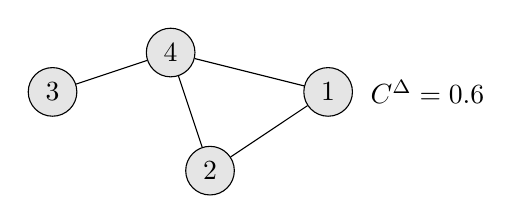
\begin{tikzpicture}
  [scale=.5,auto=left,every node/.style={circle,draw=black,fill=gray!20}]
  \node (n1) at (15,7) {1};
  \node (n2) at (12,5)  {2};
  \node (n3) at (8,7)  {3};
  \node (n4) at (11,8)  {4};
  \node[draw=none,fill=none,rectangle,right=1mm of n1] {$C^\Delta = 0.6$}; 

  \draw ({n1}) -- ({n2});
  \draw ({n3}) -- ({n4});
  \draw ({n1}) -- ({n4});
  \draw ({n2}) -- ({n4});
\end{tikzpicture}
\caption{Example Clustering Coefficient ($C^\Delta$) values for sample graphs}
\label{fig:example_graphs}
\end{figure}

\noindent\\\textit{\textbf{Small World Quotient ($Q$)}}\\
The definition of a \textit{small world} graph can be formalized by the following equations\cite{humphries2008network,uzzi2005collaboration}.

First, let $\gamma^{\Delta}_g$ equal the ratio of the clustering coefficient of a given graph and a random graph.
\[\gamma^{\Delta}_g = \frac{C^{\Delta}_g }{C^{\Delta}_{rand} } \]

Next apply a similar pattern to the average path length $\lambda_g$.
\[\lambda_g = \frac{L_g }{L_{rand} } \]

Finally, the ratio of the above calculations yields the small world quotient, or $Q$, of the graph
\[Q = \frac{\gamma^{\Delta}_g }{\lambda_g} \]

We assume for throughout that any graph exhibiting {$Q > 1$} is a small world graph.

\noindent\\\textit{\textbf{Performance}}\\
To further explore the data, a measurement of project performance was needed. As the explored datasets consisted entirely of open source projects, research indicates that \textit{quality}, \textit{use}, \textit{user satisfaction}, and \textit{impact} are possible metrics to measure performance or \textit{success}\cite{crowston2003defining}.\\

For both datasets, we base our performance metric on \textit{use}. For Freecode, we use the \textit{Popularity Score} metric, which is calculated by the following formula\footnote{http://help.freecode.com/kb/statistics/how-do-you-measure-a-projects-popularity}:

\[ ((record\ hits + URL\ hits) \cdot (followers + 1))^{1/2} \]

For the SourceForge dataset, performance is based on the repository's internal \textit{rank} metric. This metric ranks each project from 1 to the total number of projects in SourceForge ($P_{sf}$), or ${1 <= rank <= |P_{sf}|}$. At the time of this writing, no formula for the \textit{rank} metric could be located for citation.  Note that there was no attempt to normalize the two performance metrics between datasets. Because of this, no cross-dataset measurements can be made, as the performance metric is only valid in the context of the enclosing dataset. 

\subsubsection{Qualitative Analysis}
So far we have explored, via data analysis, how closely project collaborators are connected to one another, and what correlations we can derive from this analysis. We have said little as to why these connections are made, how they are maintained, and what exactly a connection means at a personal level. Via qualitative analysis, we will attempt to enrich our data analysis by providing deeper context.\\
A connection between two people is much more than an edge between two nodes in a graph. It has been asserted that people tend to make connections with people with whom they share similarities\cite{mcpherson2001birds}. This idea of homophily, however, needs to be further expanded before we can make assertions about correlations to performance. It has been shown that demographic homophily is complex to measure, correlates little to performance outcomes, and in fact correlates negatively\cite{reagans2004make,lawrence1997perspective}. For our purposes, it is much more appropriate to examine how teams best leverage similarities of knowledge and information, as the flow of these assets can be a key driver to success\cite{nissen2002extended}.\\
In the same way we can explore the role of team familiarity. The two types of familiarity that we will explore are \textit{member} familiarity and \textit{task/project} familiarity\cite{harrison2003time}. These metrics, although not captured in data, could be important factors in \textit{how} teams form, and thus help us to understand \textit{why} teams perform the way that they do.\\

To further study these factors, we arranged interviews with two current professionals in the field. Both have had experience with project management and are certified Project Management Professionals (PMP)\textregistered. We proposed to them the following questions, with the intent of expanding further the questions posed above:

\noindent\\\textit{Q1: How do development teams collaborate and share ideas?}\\
\noindent\\\textit{Q2: Do teams generally remain intact over multiple projects, or do members often shuffle and re-combine?}\\
\noindent\\\textit{Q3: When assembling a team, which is preferred -- members familiar with each other, or members familiar with the task or project.}\\
\noindent\\\textit{Q4: What are some characteristics of a high performing team?}\\
\noindent\\\textit{Q5: In your experience, is it better to (A) keep an innovative team intact, (B) periodically bring in new members or re-assign existing members, or (C) split up and disperse the team to as many other projects as possible?}\\

\section{Results}

\subsection{Quantitative}

\begin{table}[htbp]\centering
\caption{\label{fig:freecode_summary_stats}
\textbf{Freecode Statistics} }\begin{tabular} {@{} l r  r  r  r  r  r  @{}} \\ \hline
\textbf{Var} & \textbf{Mean} & \textbf{Med} & \textbf{Max} & \textbf{Min} & \textbf{Std} \\ 
\hline
$Q$ & 1.36 & 1.0 & 6.38 & 0.85 & 0.72 \\ 
$C^{\Delta}$ & 0.91 & 1.0 & 1.0 & 0.18 & 0.19 \\ 
$\overline{C^{\lambda}}$ & 0.85 & 1.0 & 1.0 & 0.14 & 0.25 \\ 
$L$ & 1.12 & 1.0 & 2.32 & 1.0 & 0.26 \\ 
N & 4.06 & 3.0 & 16.0 & 3.0 & 2.12 \\ 
E & 5.34 & 3.0 & 78.0 & 2.0 & 7.48 \\ 
\hline
\multicolumn{6}{@{}l}{
P: 41121, $P_c$: 156, C: 21970}
\end{tabular}
\end{table}

\begin{table}[htbp]\centering
\caption{\label{fig:summary_stats}
\textbf{SourceForge Statistics} }\begin{tabular} {@{} l r  r  r  r  r  r  @{}} \\ \hline
\textbf{Var} & \textbf{Mean} & \textbf{Med} & \textbf{Max} & \textbf{Min} & \textbf{Std} \\ 
\hline
$Q$ & 1.44 & 1.0 & 8.04 & 0.78 & 0.69 \\ 
$C^{\Delta}$ & 0.95 & 1.0 & 1.0 & 0.19 & 0.12 \\ 
$\overline{C^{\lambda}}$ & 0.91 & 1.0 & 1.0 & 0.08 & 0.19 \\ 
$L$ & 1.09 & 1.0 & 3.84 & 1.0 & 0.22 \\ 
N & 5.38 & 4.0 & 194.0 & 3.0 & 5.27 \\ 
E & 15.88 & 6.0 & 8778.0 & 2.0 & 100.88 \\ 
\hline
\multicolumn{6}{@{}l}{
P: 163244, $P_c$: 9532, C: 222920}
\end{tabular}
\end{table}


Summary statistics for the graph analysis are captured in figure \ref{fig:summary_stats}.  Statistics analyzed included:\\
$Q$ - \textit{Small World Quotient}\\
$C^\Delta$ - \textit{Clustering Coefficient - Transitivity}\\
$\overline{C^\lambda}$ - \textit{Clustering Coefficient - Average}\\
$L$ - \textit{Average Path Length}\\
$N$ - \textit{Number of Nodes}\\
$E$ - \textit{Number of Edges}\\
The results shown were as measured over the number of projects $P$, with the total number of contributors $C$. The number of connected subgraphs analyzed is shown as $P_c$. The connected subgraphs are the main unit of analysis, and each statistical operation is applied to the set of subgraphs $P_c$.

A mean value of $Q$ was observed to be $> 1$ for both data sets, which meets the criteria for a small world network\cite{humphries2008network}. The median, however, is 1.0 in both cases, which does not match the small world network criteria. A possible explanation of this is the power law distribution of $Q$ observed in both data sets (figures \ref{fig:q_fc_distribution} and \ref{fig:q_sf_distribution}). This indicates that a large proportion of $Q$ values are around 1.\\

$C^\Delta$ and $\overline{C^\lambda}$ both indicate values approaching 1. This observation indicates a high degree of clustering\cite{watts1998collective}. Exploring this phenomenon further, we can derive that most graphs resemble the middle or the bottom graph in figure \ref{fig:example_graphs}, with relatively few resembling the top graph.\\

Note that $P_c$ values are relatively small compared to $P$ and $C$ values. It would be intuitive to assume that {$N \times P_c \approx C$} -- in other words, if we split the entire graph into connected subgraphs, the number of subgraphs ($P_c$) multiplied by the average number of nodes ($N$) per subgraph should approximately equal the total number of contributors ($C$). This, however, is not the case. In fact, $P_c$ is notably smaller than expected. Recall that during analysis, subgraphs of {$< 3$} nodes were not considered. We can assume then that a large number of subgraphs are very small, with only one or two nodes. Further analysis is needed to fully understand the implications of this.

To validate the hypothesis, we expect to find that intermediate values of $Q$ will be correlated with more popular projects. To explore this possibility, we first compare the popularity given $Q$ values as shown in figures \ref{fig:q_fc_graph} and \ref{fig:q_sf_graph}. The $Q$ values do display the inverse U-shaped characteristic as compared to popularity, which aligns with the findings of Uzzi \textit{et. al}\cite{uzzi2005collaboration}.

\begin{figure}
\begin{center}
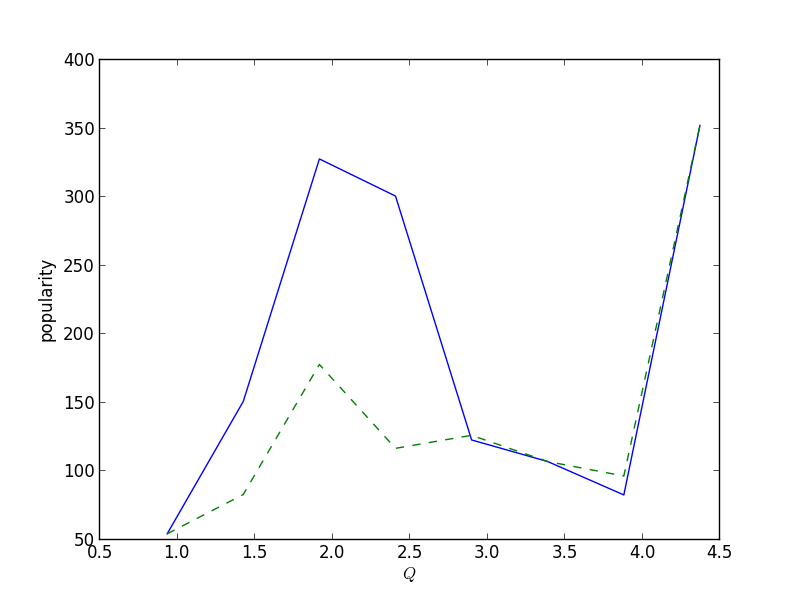
\includegraphics[width=0.5\textwidth]{images/freecode-graph.png}
\end{center}
\caption{Freecode $Q$ and Project Popularity}
\label{fig:q_fc_graph}
\end{figure}

\begin{figure}
\begin{center}
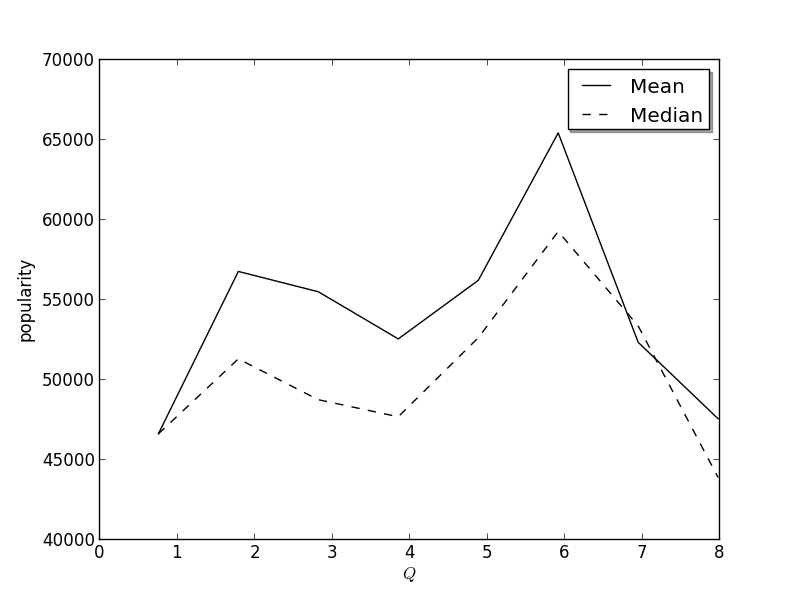
\includegraphics[width=0.5\textwidth]{images/sf-graph.png}
\end{center}
\caption{SourceForge $Q$ and Project Popularity}
\label{fig:q_sf_graph}
\end{figure}

Distribution of $Q$ values are shown in figures \ref{fig:q_fc_distribution} and \ref{fig:q_sf_distribution}. The values of $Q$ generally follow a power-law distribution, with most values being at our around {$Q = 1$}. This indicates that many graphs are close to the delineation of being considered small-world\cite{humphries2008network}.

\begin{figure}
\begin{center}
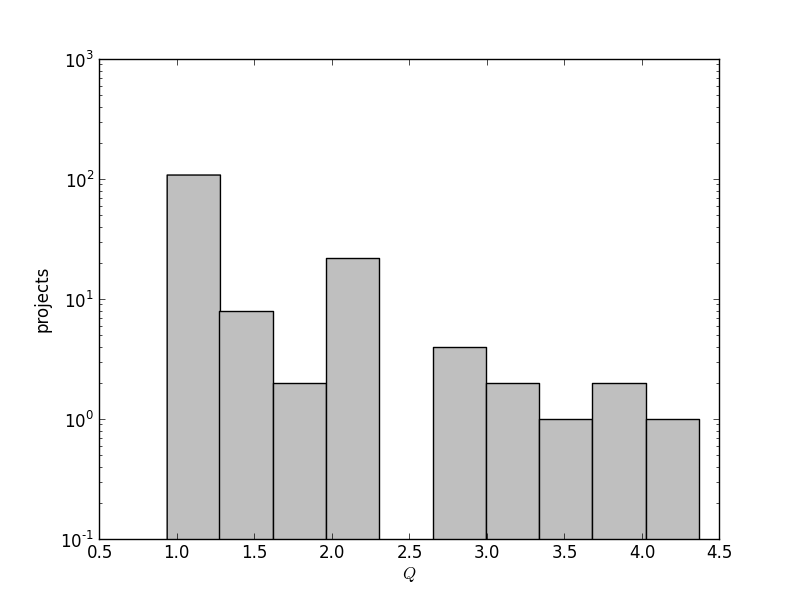
\includegraphics[width=0.5\textwidth]{images/freecode-q-histo.png}
\end{center}
\caption{Freecode $Q$ Distribution}
\label{fig:q_fc_distribution}
\end{figure}

\begin{figure}
\begin{center}
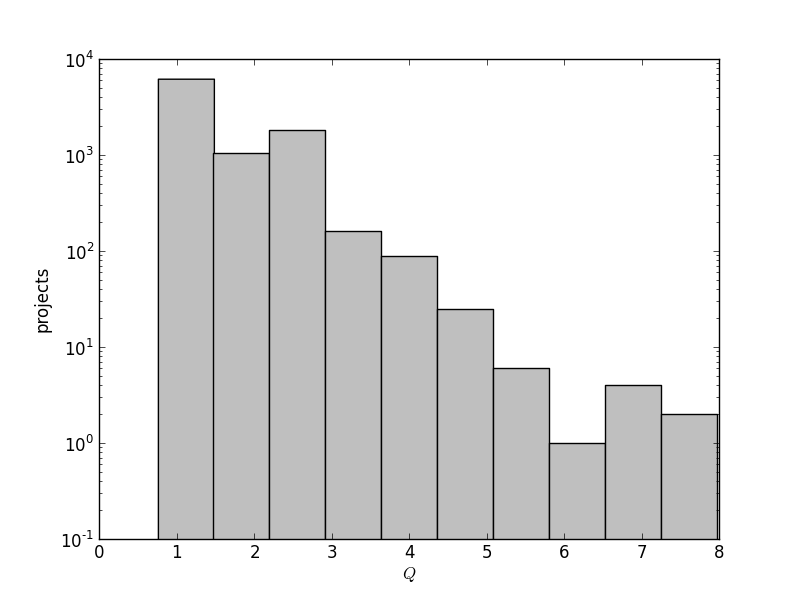
\includegraphics[width=0.5\textwidth]{images/sf-q-histo.png}
\end{center}
\caption{SourceForge $Q$ Distribution}
\label{fig:q_sf_distribution}
\end{figure}

\subsection{Qualitative}
The research interviews provided a look into how some of these quantitative findings translate into actual industry practice. They also helped us to obtain a deeper understanding of what we had found in the data analysis, as we could begin to build some workplace context into our results. There were are few re-occurring themes from which we will base our analysis\cite{stmartin_interview,rana_interview}:

\noindent\\\textit{\textbf{New contributors are good, as long as the core team remains intact.}}\\
Both participants mentioned the idea of keeping a ``core" team intact. This was certainly an often cited notion in both interviews. This concept appears to align with the idea of a \textit{core/periphery}\cite{borgatti2000models}, where the graph under study contains one (or many) tightly interconnected subgraphs, with less tightly connected nodes radiating out from this core.

Although our data analysis does not include any examination of a core/periphery, it is an interesting direction for future research. Notably, has been suggested that individual performance in a group is highest if that individual is not in the core or the periphery, but somewhere in between\cite{cattani2008core}. This is especially interesting as it aligns in principle with our hypothesis that intermediate values of $Q$ are optimal.

\noindent\\\textit{\textbf{Teams can stagnate without new members.}}\\
Both interview participants indicated that new members were essential in bringing new ideas to the team. A highly static team (or, a team with a high $Q$ value), runs the risk of falling behind the technology trends. Occasional new members (or, intermediate values of $Q$) were perceived as a positive in terms of information flow.

\noindent\\\textit{\textbf{Collaboration is key to performance.}}\\
Both interviewees suggested that team collaboration had a direct impact on performance. Teams that showed good collaboration both intra-team and inter-team were noted for their positive performance characteristics. Further exploration of this topic is needed to determine more fully the nature of this collaboration. Specifically, we know that high conflict is detrimental to team performance, especially in complex work environments\cite{de2003task}. A further research direction may be whether or not good team collaboration/communication promotes conflict avoidance, conflict resolution, or otherwise.

\noindent\\\textit{\textbf{Priority, focus, and timeline are strong drivers.}}\\
Focus was specifically called out as an indicator of performance in one interview. Clear goals and a common objective were positive influencer, while continuously shifting focus was a negative influence. Research in this area suggests that creative teams have ``goals that are clear and compelling, but also open and challenging.''\cite{isaksen2002climate}

Timeline and priority were discussed as strong factors in team success. Team building could be thought of as function of the timeline -- meaning that as the timeline of the project increased, more time could be devoted to team building activities.

It was also indicated that priority was a major factor. Different project priorities, and the resultant shifting of resources, had the possible effect of the weakening of string team's core members. This can be related to focus as well, as changing priorities can cause resource realignment and decreased overall focus.

\section{Conclusion}
Our hypothesis theorizes that medium values of clustering between collaborators on projects is optimal for project performance. The data analysis, specifically figures \ref{fig:q_fc_graph} and \ref{fig:q_sf_graph}, seem to support this claim. Also, qualitative research seems to support the hypothesis as well. Our interviews revealed that from experience, teams perform best when a stable core is periodically augmented with new members. This would be a qualitative representation of a intermediate $Q$ value -- significant clustering but not to the extent of isolation. Given both the quantitative and qualitative analysis, we can assert to align with Uzzi's findings\cite{uzzi2005collaboration} and show that intermediate values of $Q$ are correlated with increased project performance.

\section{Future Research}
Social networks, interpersonal relationships, and software development are all complex topics. We have explored a narrow slice of these in context, and there are some important areas of future exploration. First, the contributor graph contains a large amount of subgraphs, and as a whole appears less clustered than some other observed social network graphs -- consistent with Madey's findings\cite{madey2002open} on SourceForge data. As noted in our analysis, a large number of these subgraphs have only one or two contributors. This implies that a large number of contributors work alone and on a single project. We do not, with the current analysis, know how (or if) this degrades the quality of our findings.\\

A further area of study would be how our findings relate to previously defined \textit{success factors} in projects\cite{cooke2002real}. Also, we do not know directly \textit{how} intermediate values of $Q$ influence performance -- we can only observe a quantitative and qualitative correlation. We make a tacit equivalence to clustering and knowledge sharing, but we have not directly observed that in our analysis. Research does suggest that social factors are knowledge sharing motivators\cite{hendriks1999share}, but how that relates specifically to our work is unexplored here.\\

\section{Acknowledgments}
We thank Praveen Mittal and John Kaman for their insight, guidance, and instruction, M Iftekhar (Ifte) Rana and Traci St. Martin for their time and expertise, and Rick Kiefer for his review.

\bibliographystyle{plain}
\bibliography{bibliography}

\clearpage

\section*{Appendix A: Interview Transcript}
Interview with Traci St. Martin, PMP\textregistered, Mayo Clinic, Nov 21, 2013.

\subsection*{Q1: How do development teams collaborate and share ideas?}
Co-location is important for teams, as it really fosters communication and collaboration. Being able to quickly talk with someone and resolve a problem is very important. In some cases, having the team in the same room is beneficial, especially if the project is going badly. That way, ideas can get discussed and problems resolved very quickly. Regular meetings are also important with large teams. With these meetings, it is important to have the correct tools to facilitate communication. These meetings help projects have visibility into each other. Management support is essential to this communication process. Meetings between teams can consist of all members of the teams if the teams are small enough, but most of the time should just be a representative.

\subsection*{Q2: Do teams generally remain intact over multiple projects, or do members often shuffle and re-combine?}
I have had both. It really depends on the projects and the situation at the time. It can be nice to have new people brought in to make things different, and to bring some new thoughts and ideas to the team. Even one person can change the dynamics of a team, either positively or negatively. As a project manager, I have to be watchful of this, as negativity can spread quickly. I have also noticed that as people move around to different projects, they are generally brought up to the level of the team. For example, if somebody joins a high performing team, they tend to elevate their skill to match that of the group, which is a good thing.

\subsection*{Q3: When assembling a team, which is preferred -- members familiar with each other, or members familiar with the task or project?}
Familiarity is good, but you have to account for burnout if people work on the same project for too long. This really depends on project dynamics, special skills needed, etc. It is important to note, however, that team members can be familiar with each other but not get along well, or not work well with each other. I have had projects where team members were very familiar with each other, but did not function well as a team. Clashing personalities and other team problems can cause a toxic environment. Most importantly, whether the team is familiar with each other or not, is that they can share knowledge and skills.

\subsection*{Q4: What are some characteristics of a high performing team?}
Most teams I notice go through the Forming, Storming, Norming and Performing stages. Good teams usually have a strong leader, a good vision, and good management support. Of course, they also possess the necessary skills for the project (or, if not, are willing to learn). Good teams have respect for each other, their leadership, and their management. Professionalism is also an indicator of a high performing team. Teams that truly care about their job, the team, and the project are generally more successful. Teams are generally more successful if the individuals themselves are skilled and talented. Being able to react to change is important, and good teams generally have good change management procedures.

\subsection*{Q5: In your experience, is it better to (A) keep an innovative team intact, (B) periodically bring in new members or re-assign existing members, or (C) split up and disperse the team to as many other projects as possible?}
In general, I like to keep good teams intact. It is, however, nice to bring in or add a new member to a team. One strategy I like to employ is to bring in a new member, train them and let them learn from the high performing team, and move them out of the project and into a new one. This keeps the core team intact, which is important. Priorities can greatly influence this, and sometimes personnel moves are driven from higher management priorities. If experts are removed from a high performing team, the team may suffer. This is, however, a risk that knowledge becomes concentrated. High priority/high visibility teams have a tendency to get the highest performing individuals, which can cause other projects to suffer. 
\clearpage

\section*{Appendix B: Interview Transcript}
Interview with M Iftekhar (Ifte) Rana, PMP\textregistered, Mayo Clinic, Nov 26, 2013.

\subsection*{Q1: How do development teams collaborate and share ideas?}
In my previous experiences, there were tight dependencies between teams and changes could have large impacts. Because of this, team collaboration was important and was stressed. Because of the tight dependencies, teams were involved in each other's planning phases. We found that bringing teams together during planning helped collaboration and communication. Also, we noticed that the quality of communication and collaboration between teams had a direct impact how how teams performed, and how the project faired as a whole.


\subsection*{Q2: Do teams generally remain intact over multiple projects, or do members often shuffle and re-combine?}
It is more of a problem when focus changes rapidly. If there is a stable focus for the project, and the goals of the project remain relatively intact, shifting of personnel has less impact. Continuously changing focus definitely has a negative impact on team performance. Also, when focus is changing rapidly, it is hard to maintain a stable team core, as they tend to get reassigned or loaned out to different projects.


\subsection*{Q3: When assembling a team, which is preferred -- members familiar with each other, or members familiar with the task or project?}
This really depends on the time-line of the project. Short-term projects don't have as much time for team bonding -- it is more important to get the people with the right skill set. For longer term projects, you have to be much more careful about people getting along with each other. For these types of projects, you can afford to invest some time into getting the team right and doing some team building. Also, with long term projects, you have more of a chance of members ``learning on the job," so even if the technical skills aren't there right away, you can factor in some learning time if they are a good fit personality-wise. It is the same reason why we ask a lot of behavioral questions for new full-time employees, and less so with contractors. It all depends on the time commitment and how much team building you can plan for.


\subsection*{Q4: What are some characteristics of a high performing team?}
The number one most important factor for a high performing team is good communication skills. Good teams that I've worked are highly connected, and all members of the team communication with each other. This leads to feedback coming from many different angles, which helps teams get better. Team performance is usually tied directly to how well a team communicates and shares knowledge with each other.


\subsection*{Q5: In your experience, is it better to (A) keep an innovative team intact, (B) periodically bring in new members or re-assign existing members, or (C) split up and disperse the team to as many other projects as possible?}
It is usually good to keep teams intact if they are performing well. That said, if you do not keep growing the team, they will quickly lose touch with changes in technology. New members help to bring this into the team, and if a team is isolated they often don't keep up. Technology trends move very quickly, so it is essential to have fast communication channels so that information can spread quickly. Even if new/different members aren't coming into the team, there still should be communication channels open. Communication between teams should happen whether or not teams are actually working together. In general, it is best to periodically bring in new members, but keep the core team intact if possible.

\end{document}